\documentclass[journal,12pt,twocolumn]{IEEEtran}
%
\usepackage{setspace}
\usepackage{gensymb}
%\doublespacing
\singlespacing

%\usepackage{graphicx}
%\usepackage{amssymb}
%\usepackage{relsize}
\usepackage[cmex10]{amsmath}
%\usepackage{amsthm}
%\interdisplaylinepenalty=2500
%\savesymbol{iint}
%\usepackage{txfonts}
%\restoresymbol{TXF}{iint}
%\usepackage{wasysym}
\usepackage{amsthm}
\usepackage{mathrsfs}
\usepackage{txfonts}
\usepackage{stfloats}
\usepackage{steinmetz}
\usepackage{bm}
\usepackage{cite}
\usepackage{cases}
\usepackage{subfig}
%\usepackage{xtab}
\usepackage{longtable}
\usepackage{multirow}
%\usepackage{algorithm}
%\usepackage{algpseudocode}
\usepackage{enumitem}
\usepackage{mathtools}
\usepackage{tikz}
\usepackage{circuitikz}
\usepackage{verbatim}
\usepackage{tfrupee}
\usepackage[breaklinks=true]{hyperref}
%\usepackage{stmaryrd}
\usepackage{tkz-euclide} % loads  TikZ and tkz-base
%\usetkzobj{all}
\usepackage{listings}
    \usepackage{color}                                            %%
    \usepackage{array}                                            %%
    \usepackage{longtable}                                        %%
    \usepackage{calc}                                             %%
    \usepackage{multirow}                                         %%
    \usepackage{hhline}                                           %%
    \usepackage{ifthen}                                           %%
  %optionally (for landscape tables embedded in another document): %%
    \usepackage{lscape}     
\usepackage{multicol}
\usepackage{chngcntr}
%\usepackage{enumerate}

%\usepackage{wasysym}
%\newcounter{MYtempeqncnt}
\DeclareMathOperator*{\Res}{Res}
%\renewcommand{\baselinestretch}{2}
\renewcommand\thesection{\arabic{section}}
\renewcommand\thesubsection{\thesection.\arabic{subsection}}
\renewcommand\thesubsubsection{\thesubsection.\arabic{subsubsection}}

\renewcommand\thesectiondis{\arabic{section}}
\renewcommand\thesubsectiondis{\thesectiondis.\arabic{subsection}}
\renewcommand\thesubsubsectiondis{\thesubsectiondis.\arabic{subsubsection}}

% correct bad hyphenation here
\hyphenation{op-tical net-works semi-conduc-tor}
\def\inputGnumericTable{}                                 %%

\lstset{
%language=C,
frame=single, 
breaklines=true,
columns=fullflexible
}
%\lstset{
%language=tex,
%frame=single, 
%breaklines=true
%}

\begin{document}
%


\newtheorem{theorem}{Theorem}[section]
\newtheorem{problem}{Problem}
\newtheorem{proposition}{Proposition}[section]
\newtheorem{lemma}{Lemma}[section]
\newtheorem{corollary}[theorem]{Corollary}
\newtheorem{example}{Example}[section]
\newtheorem{definition}[problem]{Definition}
%\newtheorem{thm}{Theorem}[section] 
%\newtheorem{defn}[thm]{Definition}
%\newtheorem{algorithm}{Algorithm}[section]
%\newtheorem{cor}{Corollary}
\newcommand{\BEQA}{\begin{eqnarray}}
\newcommand{\EEQA}{\end{eqnarray}}
\newcommand{\define}{\stackrel{\triangle}{=}}
\bibliographystyle{IEEEtran}
%\bibliographystyle{ieeetr}
\providecommand{\mbf}{\mathbf}
\providecommand{\pr}[1]{\ensuremath{\Pr\left(#1\right)}}
\providecommand{\qfunc}[1]{\ensuremath{Q\left(#1\right)}}
\providecommand{\sbrak}[1]{\ensuremath{{}\left[#1\right]}}
\providecommand{\lsbrak}[1]{\ensuremath{{}\left[#1\right.}}
\providecommand{\rsbrak}[1]{\ensuremath{{}\left.#1\right]}}
\providecommand{\brak}[1]{\ensuremath{\left(#1\right)}}
\providecommand{\lbrak}[1]{\ensuremath{\left(#1\right.}}
\providecommand{\rbrak}[1]{\ensuremath{\left.#1\right)}}
\providecommand{\cbrak}[1]{\ensuremath{\left\{#1\right\}}}
\providecommand{\lcbrak}[1]{\ensuremath{\left\{#1\right.}}
\providecommand{\rcbrak}[1]{\ensuremath{\left.#1\right\}}}
\theoremstyle{remark}
\newtheorem{rem}{Remark}
\newcommand{\sgn}{\mathop{\mathrm{sgn}}}
\providecommand{\abs}[1]{\left\vert#1\right\vert}
\providecommand{\res}[1]{\Res\displaylimits_{#1}} 
\providecommand{\norm}[1]{\left\lVert#1\right\rVert}
%\providecommand{\norm}[1]{\lVert#1\rVert}
\providecommand{\mtx}[1]{\mathbf{#1}}
\providecommand{\mean}[1]{E\left[ #1 \right]}
\providecommand{\fourier}{\overset{\mathcal{F}}{ \rightleftharpoons}}
%\providecommand{\hilbert}{\overset{\mathcal{H}}{ \rightleftharpoons}}
\providecommand{\system}{\overset{\mathcal{H}}{ \longleftrightarrow}}
	%\newcommand{\solution}[2]{\textbf{Solution:}{#1}}
\newcommand{\solution}{\noindent \textbf{Solution: }}
\newcommand{\cosec}{\,\text{cosec}\,}
\providecommand{\dec}[2]{\ensuremath{\overset{#1}{\underset{#2}{\gtrless}}}}
\newcommand{\myvec}[1]{\ensuremath{\begin{pmatrix}#1\end{pmatrix}}}
\newcommand{\mydet}[1]{\ensuremath{\begin{vmatrix}#1\end{vmatrix}}}
%\numberwithin{equation}{section}
\numberwithin{equation}{subsection}
%\numberwithin{problem}{section}
%\numberwithin{definition}{section}
\makeatletter
\@addtoreset{figure}{problem}
\makeatother
\let\StandardTheFigure\thefigure
\let\vec\mathbf
%\renewcommand{\thefigure}{\theproblem.\arabic{figure}}
\renewcommand{\thefigure}{\theproblem}
%\setlist[enumerate,1]{before=\renewcommand\theequation{\theenumi.\arabic{equation}}
%\counterwithin{equation}{enumi}
%\renewcommand{\theequation}{\arabic{subsection}.\arabic{equation}}
\def\putbox#1#2#3{\makebox[0in][l]{\makebox[#1][l]{}\raisebox{\baselineskip}[0in][0in]{\raisebox{#2}[0in][0in]{#3}}}}
     \def\rightbox#1{\makebox[0in][r]{#1}}
     \def\centbox#1{\makebox[0in]{#1}}
     \def\topbox#1{\raisebox{-\baselineskip}[0in][0in]{#1}}
     \def\midbox#1{\raisebox{-0.5\baselineskip}[0in][0in]{#1}}
\vspace{3cm}
\title{
ASSIGNMENT 4 - EE5600
	}
\author{ RS Girish - EE20RESCH14005$^{*}$% <-this % stops a space
	}	

\maketitle
\newpage
\tableofcontents
\bigskip
\renewcommand{\thefigure}{\theenumi}
\renewcommand{\thetable}{\theenumi}

\begin{abstract}
This paper contains solution to problem no 4.8 of Linear Programming .
Links to Python codes are available below.  
\end{abstract}
Download python codes using 
\begin{lstlisting}
https://github.com/rsgirishkumar/Assignment4/codes/
\end{lstlisting}
\section{Problem}
Minimise Z=x+2y
subject to 2x+y$\geq$3, x+2y$\geq$6, x,y$\geq$0.\\
Show that the minimum of Z occurs at more than two points.\\
\section{Solution}
\subsection{Theory}
Here, to minimize the above given objective function, simplex method can be used.\\
\\
The simplex algorithm for minimization problems works by converting the problem to a maximization problem, by forming an augmented matrix which includes given objective function in last row and constraints in above rows. It is transposed and then maximization is applied for the augmented matrix formed from those equations after transposing.
\\
\subsection{Solution part}
Given objective function
\begin{align}
f(x,y) = Z = x+2y
\end{align}
subject to\\
\begin{align}
2x+y\geq 3\\
x+2y\geq 6\\
x,y\geq 0
\end{align}
The matrix form of given objective function and constraints is given as below
\begin{align}
\myvec{2 & 1 & 3\\1 &2 &6\\1 & 2 &0}
\end{align}
After transposing the above matrix, we get
\begin{align}
\myvec{2 & 1 & 1\\1 &2 &2\\3&6&0}
\end{align} 
As per above transposed matrix, the constraints and objective function are as below.
\begin{align}
f(x,y) = Z = 3x+6y
\end{align}
subject to\\
\begin{align}
2x+y\geq 1\\
x+2y\geq 2\\
x,y\geq 0
\end{align}
Apply Maximization now.\\
Adding slack variables s1, s2, the inequalities can be re-written as below.
\begin{equation}
f(x,y) = Z = 3x+6y\Rightarrow Z-3x-6y=0\\
\end{equation}
\begin{equation}
2x+y\geq 1\Rightarrow 2x+y+s1=1\\
\end{equation}
\begin{equation}
x+2y\geq 2\Rightarrow x+2y+s2=2\\
\end{equation}
The augmented matrix that can be formed using objective function and constraints is given as below.
\begin{align}
\myvec{1 & -3 & -6 & 0 & 0 & 0\\0 & 2 & 1 & 1 & 0 & 1\\0 & 1 & 2 & 0 & 1 & 2}
\end{align}
Here x and y are non-basic variables. s1, s2 are basic variables. Selecting x as entering variable.\\
Entering through x in row(1).\\
Reducing augmented matrix for eliminating x in row(1) through row(2) and row(3).
\begin{align}
\myvec{1 & -3 & -6 & 0 & 0 & 0\\0 & 2 & 1 & 1 & 0 & 1\\0 & 1 & 2 & 0 & 1 & 2}
\xleftrightarrow[]{R_1 \leftarrow {R_1+R_2+R_3}}\\
\xleftrightarrow[]{R_3 \leftarrow {R_2-2R_3}}\\
\myvec{1 & 0 & -3 & 1 & 1 & 3\\0 & 2 & 1 & 1 & 0 & 1\\0 & 0 & -3 & 1 & -2 & -3}
\end{align}
eliminating x in row(1) through row(1).
\begin{align}
\xleftrightarrow[]{R_2 \leftarrow {R_2/2}}\\
\myvec{1 & 0 & -3 & 1 & 1 & 3\\0 & 1 & \frac{1}{2} & \frac{1}{2} & 0 & \frac{1}{2}\\0 & 0 & -3 & 1 & -2 & -3}
\end{align}
Here, the feasible solution may not be obtained since row(1) contains negative coefficients of non-basic variables. Hence the entering variable has to be changed to y(another non-basic variable).
Entering through y in row(2) since ratio $\frac{1}{1}$ a positive number and minimum.\\
Reducing augmented matrix for eliminating y in row(1), row(2) through row(2) and row(3).
\begin{align}
\myvec{1 & -3 & -6 & 0 & 0 & 0\\0 & 2 & 1 & 1 & 0 & 1\\0 & 1 & 2 & 0 & 1 & 2}\\
\xleftrightarrow[]{R_1 \leftarrow {R_1+3R_3}}\\
\xleftrightarrow[]{R_2 \leftarrow {2R_3-R_2}}\\
\myvec{1 & 0 & 0 & 0 & 3 & 6\\0 & 0 & 3 & -1 & 2 & 3\\0 & 1 & 2 & 0 & 1 & 2}
\end{align}
Here, the feasible solutions may be obtained as below and there may be multiple optimal solutions for Z since the row(1) contain zero coefficients of non-basic variables i.e. Z can take any any values of x and y. Hence, the objective function may have multiple minima points.
\begin{align}
\Rightarrow (x,y)=(0,0)\\
\Rightarrow Z=x+2y\\
\Rightarrow Z=0+0=0
\end{align}

This Problem can be represented in matrix form as follows,\\
    \begin{align}
        \min_{\vec{x}} Z &= \myvec{1 & 2}\vec{x}\\
        s.t. \quad 
        \myvec{
        2 & 1\\
        1 & 2
        }
        \vec{x} &\succeq \myvec{3\\6} \\
        \vec{x} &\succeq \vec{0}\\
        \vec{y} &\succeq \vec{0}
    \end{align}
The output as obtained through Python implementation:
\begin{align}
    \vec{x} = \myvec{6.89748716e-11\\5.47282454e-10}, Z = 1.16353978e-09
    \end{align}
 \begin{figure}
 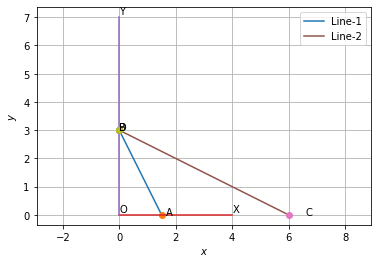
\includegraphics[width=\linewidth]{minimize.png}
  \caption{Python plot .}
  \label{fig:Fig3}
 \end{figure}
\end{document}
